%----------------------------------------------------------------------------------------
%	PACKAGES AND DOCUMENT CONFIGURATIONS
%----------------------------------------------------------------------------------------

\documentclass[12pt,a4paper]{article}

\usepackage[version=3]{mhchem} % Package for chemical equation typesetting
\usepackage{siunitx} % Provides the \SI{}{} and \si{} command for typesetting SI units
\usepackage{graphicx} % Required for the inclusion of images
\usepackage{natbib} % Required to change bibliography style to APA
\usepackage{amsmath} % Required for some math elements 
\usepackage{geometry}
\usepackage{enumerate}
\usepackage{float}
\usepackage{subfigure}
\usepackage{pdfpages}
\usepackage{siunitx}
\usepackage{fancyhdr}
\usepackage{textcomp}
\usepackage{gensymb}
\usepackage{longtable}

\includepdfset{pagecommand={\thispagestyle{fancy}}}%page number for pdf

\renewcommand{\labelenumi}{\alph{enumi}.} % Make numbering in the enumerate environment by letter rather than number (e.g. section 6)
\geometry{left=2cm,right=2cm,top=3cm,bottom=3cm}

%\usepackage{times} % Uncomment to use the Times New Roman font

%----------------------------------------------------------------------------------------
%	DOCUMENT INFORMATION
%----------------------------------------------------------------------------------------


\begin{document}

\begin{center}
~\\
\rule[0mm]{400pt}{0.5pt}
\Large{ \textsc{\newline\\UM-SJTU Joint Institute\\Physics Laboratory\\(Vp241)\\}}
\rule[0mm]{400pt}{0.5pt}
\Large{ \textsc{\newline\newline\newline\newline\newline\newline\\
Laboratory Report\\}}
\Large{\textsc{ \\ Exercise 4  \\ Polarization of Light} }

\end{center}

\begin{description}
    \item[] 
    \item[] 
    \item[] 
    \item[] 
    \item[] 
    \item[]\qquad \qquad \textbf{Name: Han Yibei \qquad ID:519370910123   \qquad    Group:11}\\
    \item[\qquad \qquad Name: Lu Xinyi \qquad ID:519370910122   \qquad    Group:11\\] 
    \item[]\qquad \qquad Date: \today
\end{description}

\newpage

%----------------------------------------------------------------------------------------
%	SECTION 1
%----------------------------------------------------------------------------------------

\section{Abstract}
In order to understand the solar cell, we did this experiment. We have tested the following cases: one cell at different distances, series cells, and parallel cells. For them, there will be I-U, P-U and P-R curves. We can found that distance and connecting method will have influence on the cell. The ff tested is about 0.637$\pm$0.012 and 0.65$\pm$0.04. Also, $\eta$ is about 4.0\%$\pm$0.3\% and 3.2\%$\pm$0.6\%. Through these analysis, we can get the preliminary understanding of solar cell.

\section{Introduction}
\subsection{Motivation}
The solar cell is useful at various of fields. In some inland regions, such as GanSu and ShanXi, solar energy is abundant because of long-time sunny days. To use environmental-friendly energy, we should have some basic understanding of the solar cell. Find out its most efficient and effective use method through this experiment may help us fulfill part of the goal.

\subsection{Theoretical Background}
Solar cells are used to turn solar energy into electic energy that we can use.

\subsubsection{Solar Cell Structure}
The most common solar cell is crystalline silicon. From Figure1, we can find that there exist n/p homo-junctions, the n-type part is thin while the p-type part is thick and they share the same surface area. There exists some metallic bars to act as electode. An anti-reflective regularly used to help decrease the reflecting loss energy.
\begin{figure}[H]
    \centering
    \includegraphics[width=12cm]{structure.png}
    \caption{Structure of a crystalline silicon solar cell   [1]}
\end{figure}

\subsubsection{Photovoltaic Effect}
When the light of appropriate strength incident the solar cell. Certain potential difference will occur because of the diffusion of minority carriers. And the current direction is from n to p.

\subsubsection{Solar Cell Parameters}
The generated $I_{ph}$ and an opposite current called "forward diode current ${I}_{D}$"[1]. So, the net current can be determined as
\begin{equation}
    {I=I}_{ph}-I_D=I_{ph}-I_0\left[e^\frac{qV_D}{nk_BT}-1\right]~~~~[1]
\end{equation}
"$V_D$ is junction voltage, $I_0$ is the diode inverse saturation current, $I_{ph}$ is the photocurrent."[1] n ranges from 1 to 2,. q is the charge of electron, $k_B$ is the Boltzmann’s constant, and T is temperature(K). So, we can rewrite the equation as
\begin{equation*}
    {I=I}_{ph}-I_0\left[e^\frac{qV}{nk_BT}-1\right]~~~~[1]
\end{equation*}
We can deduce that short-circuit current is ${I_c=I}_{ph}[1]$ as well as the open-circuit voltage is
\begin{equation*}
    V_{oc}=\frac{nk_BT}{q}ln(\frac{I_{sc}}{I_0}+1)~~~~[1]
\end{equation*}
For some load resistance $R_{m}$, we can  ${P}_m$ is $P_m=I_mV_m$. Then we can get $FF=\frac{P_m}{V_{oc}I_{sc}}=\frac{V_mI_m}{V_{oc}I_{sc}}[1]$. Also, energy conversion efficiency $\eta$ is  $\eta=\frac{P_m}{P_{in}}\times100\%[1]$.
$P_{in}$ is the "total incident radiant power"[1].
\begin{figure}[H]
    \centering
    \includegraphics[width=10cm]{characteristic.png}
    \caption{The current-voltage characteristics of a solar cell    [1]}
\end{figure}

\begin{table}[H]
    \centering
    \begin{tabular}{|c|c||c|c|c|c|}\hline
    \multicolumn{6}{|c|}{Uncertainty of $T^2$[$s^2$]}\\\hline 
    \multicolumn{2}{|c||}{horizontal}&\multicolumn{2}{c|}{incline 1}&\multicolumn{2}{c|}{incline 2}\\\hline
    $m_1$&0.00002 &$m_1$& 0.00002 & $m_1$&0.00002 \\\hline
    $m_2$&0.00003 & $m_2$&0.00003 & $m_2$&0.00003 \\\hline
    $m_3$&0.00003 &$m_3$& 0.00003 & $m_3$&0.00003 \\\hline
    $m_4$&0.00003 & $m_4$&0.00003 & $m_4$&0.00003 \\\hline
    $m_5$&0.00003 & $m_5$&0.00003 & $m_5$&0.00003 \\\hline
    $m_6$&0.00003 & $m_6$&0.00003 & $m_6$&0.00003\\\hline
    \end{tabular}
    \caption{Uncertainty of $T^2$}
    \label{Tsquare}
\end{table}

\subsubsection{Solar Cell Equivalent Circuit}
In Fig.3, a solar cell can be thought as a circuit with the current
\begin{equation*}
    I=I_{ph}-I_0\{exp[\frac{q(V+R_sI)}{nk_BT}]-1\}-\frac{V+R_sI}{R_{sh}}~~~~[1]
\end{equation*}
To have higher efficiency, we should have small $R_s$ as well as large $R_{sh}$.
\begin{figure}[H]
    \centering
    \includegraphics[width=8cm]{equivalent.png}
    \caption{Solar cell equivalent circuit~~~~[1]}
\end{figure}


\section{Discription of Experiment}
\subsection{Apparatus}
The setup consists of "a photovoltaic device(5W), a 300W tungsten-halogen lamp serving as a radiation source, two digital multimeters, two adjustable resistors, a solar power meter, a wiring board and a measuring tape."[1]
\begin{figure}[H]
    \centering
    \subfigure{
        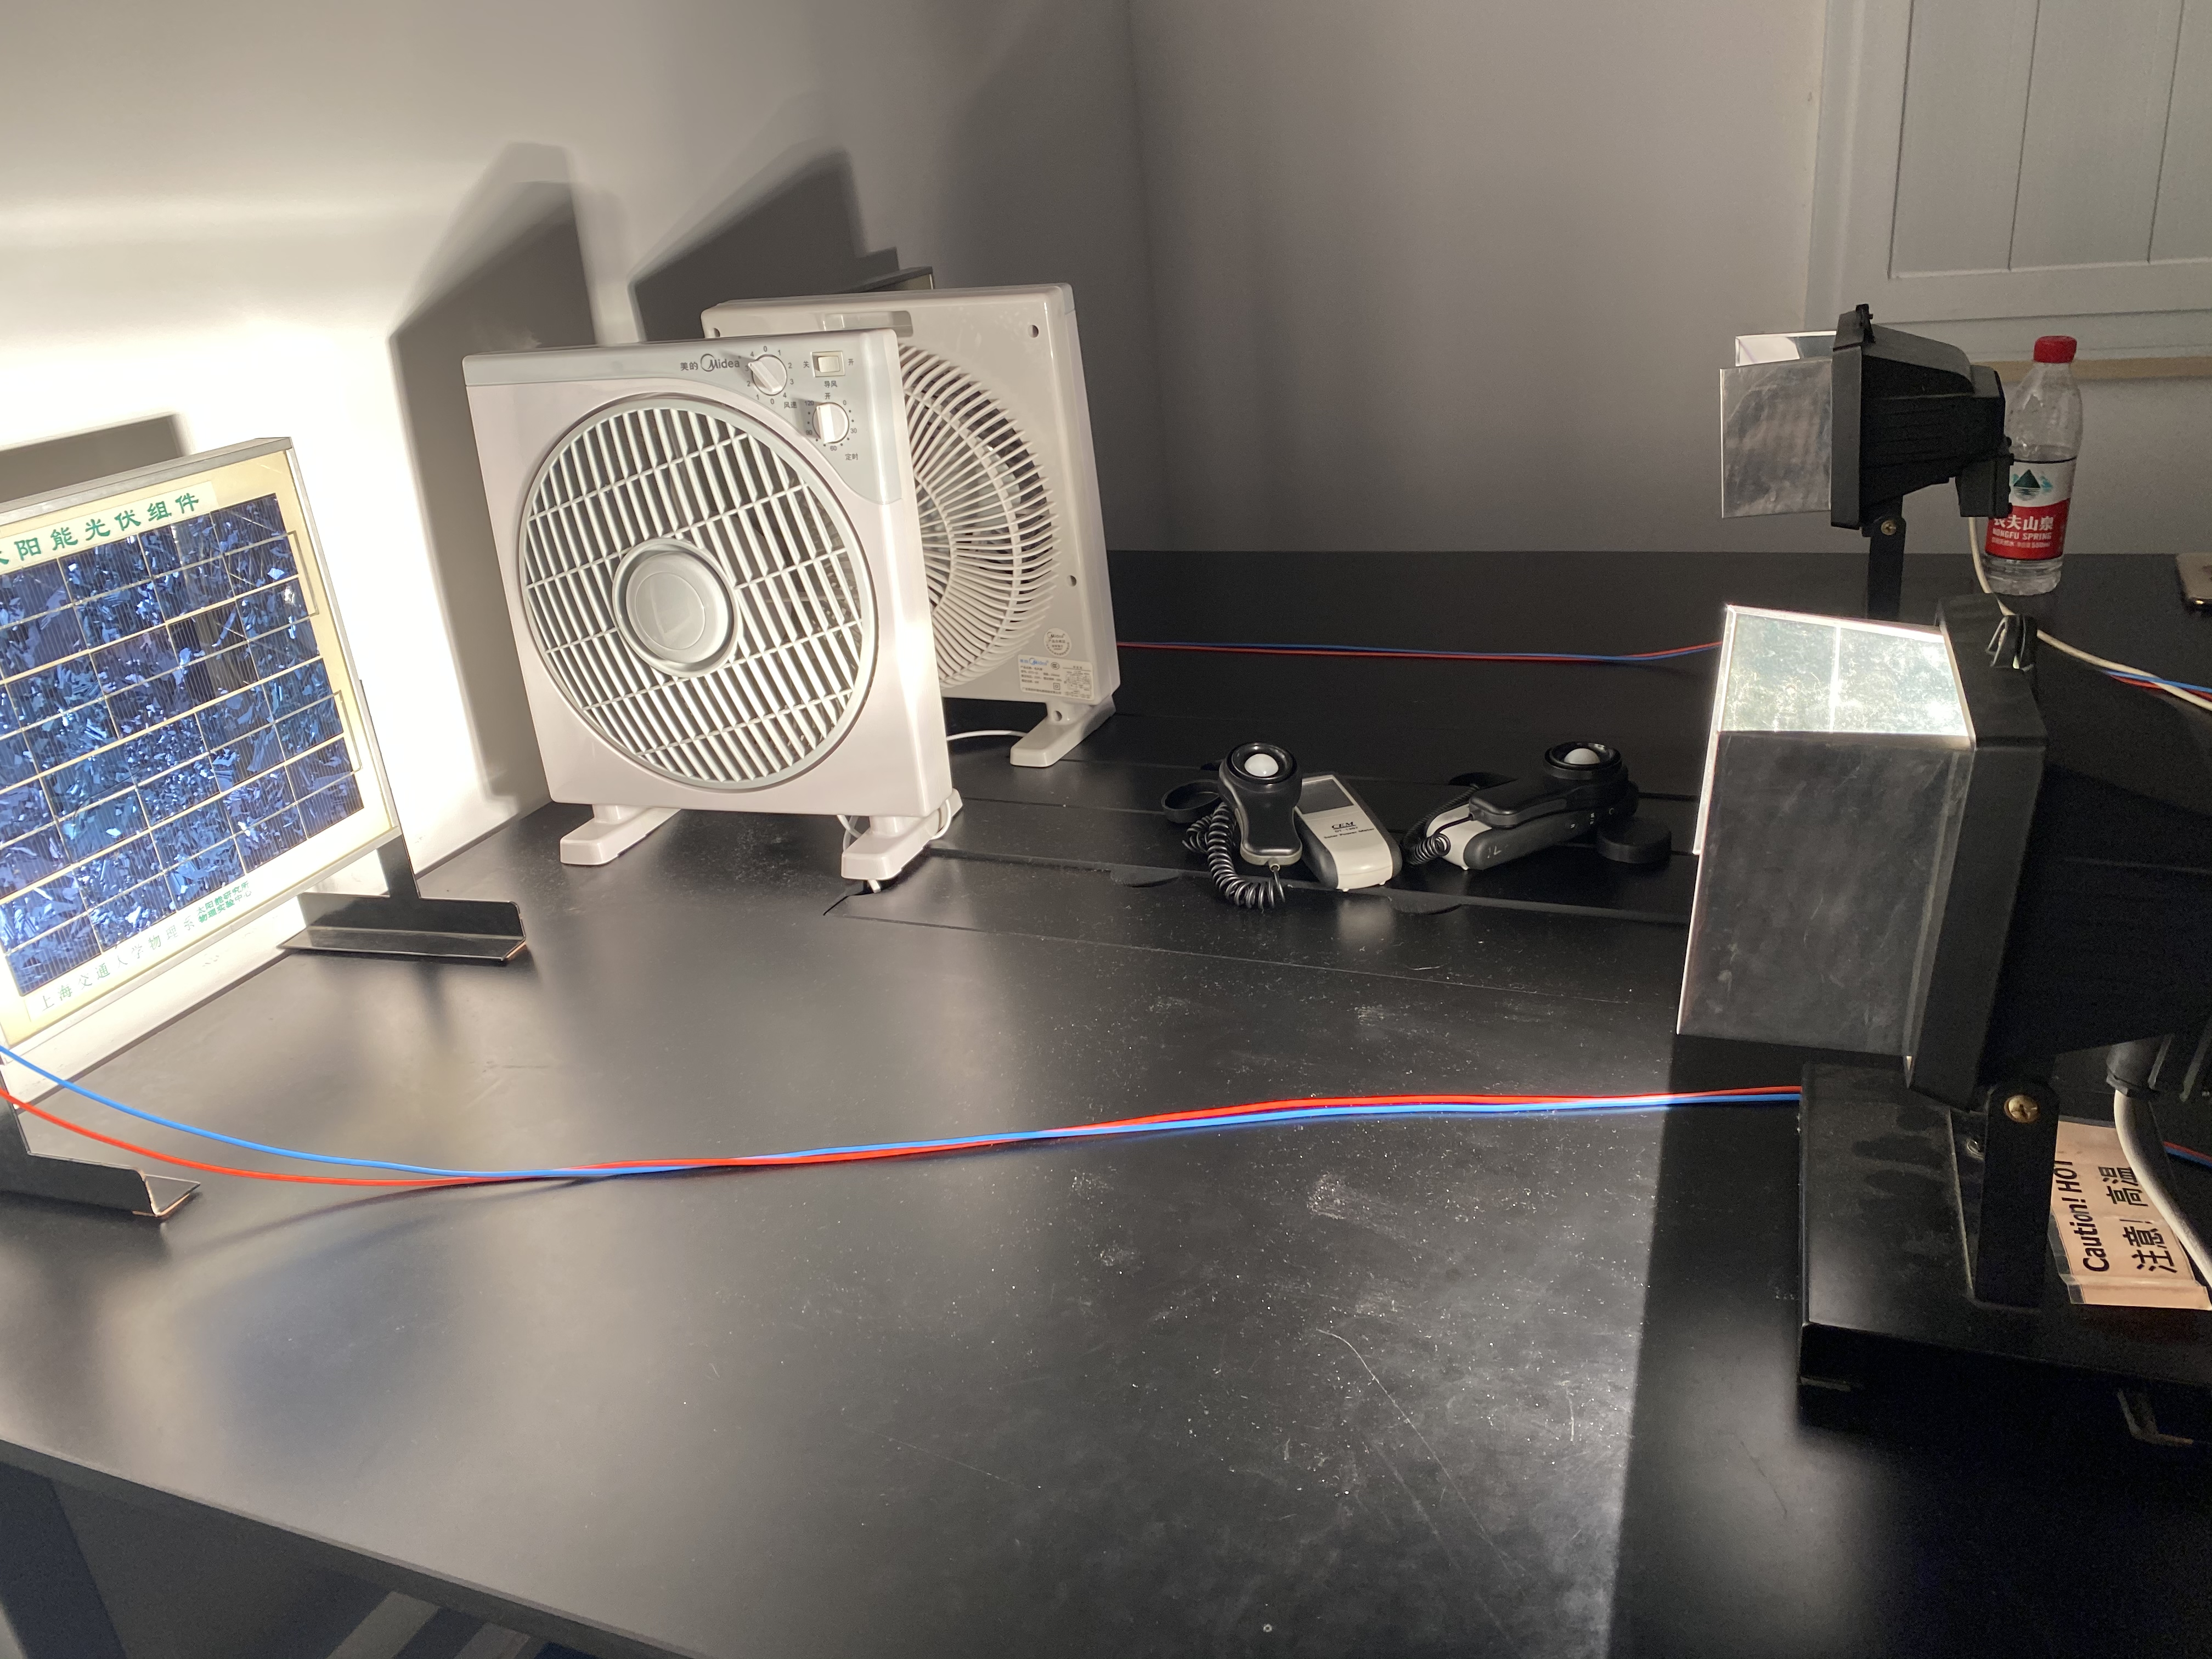
\includegraphics[width=6cm]{app.jpg}
    }
    \subfigure{
        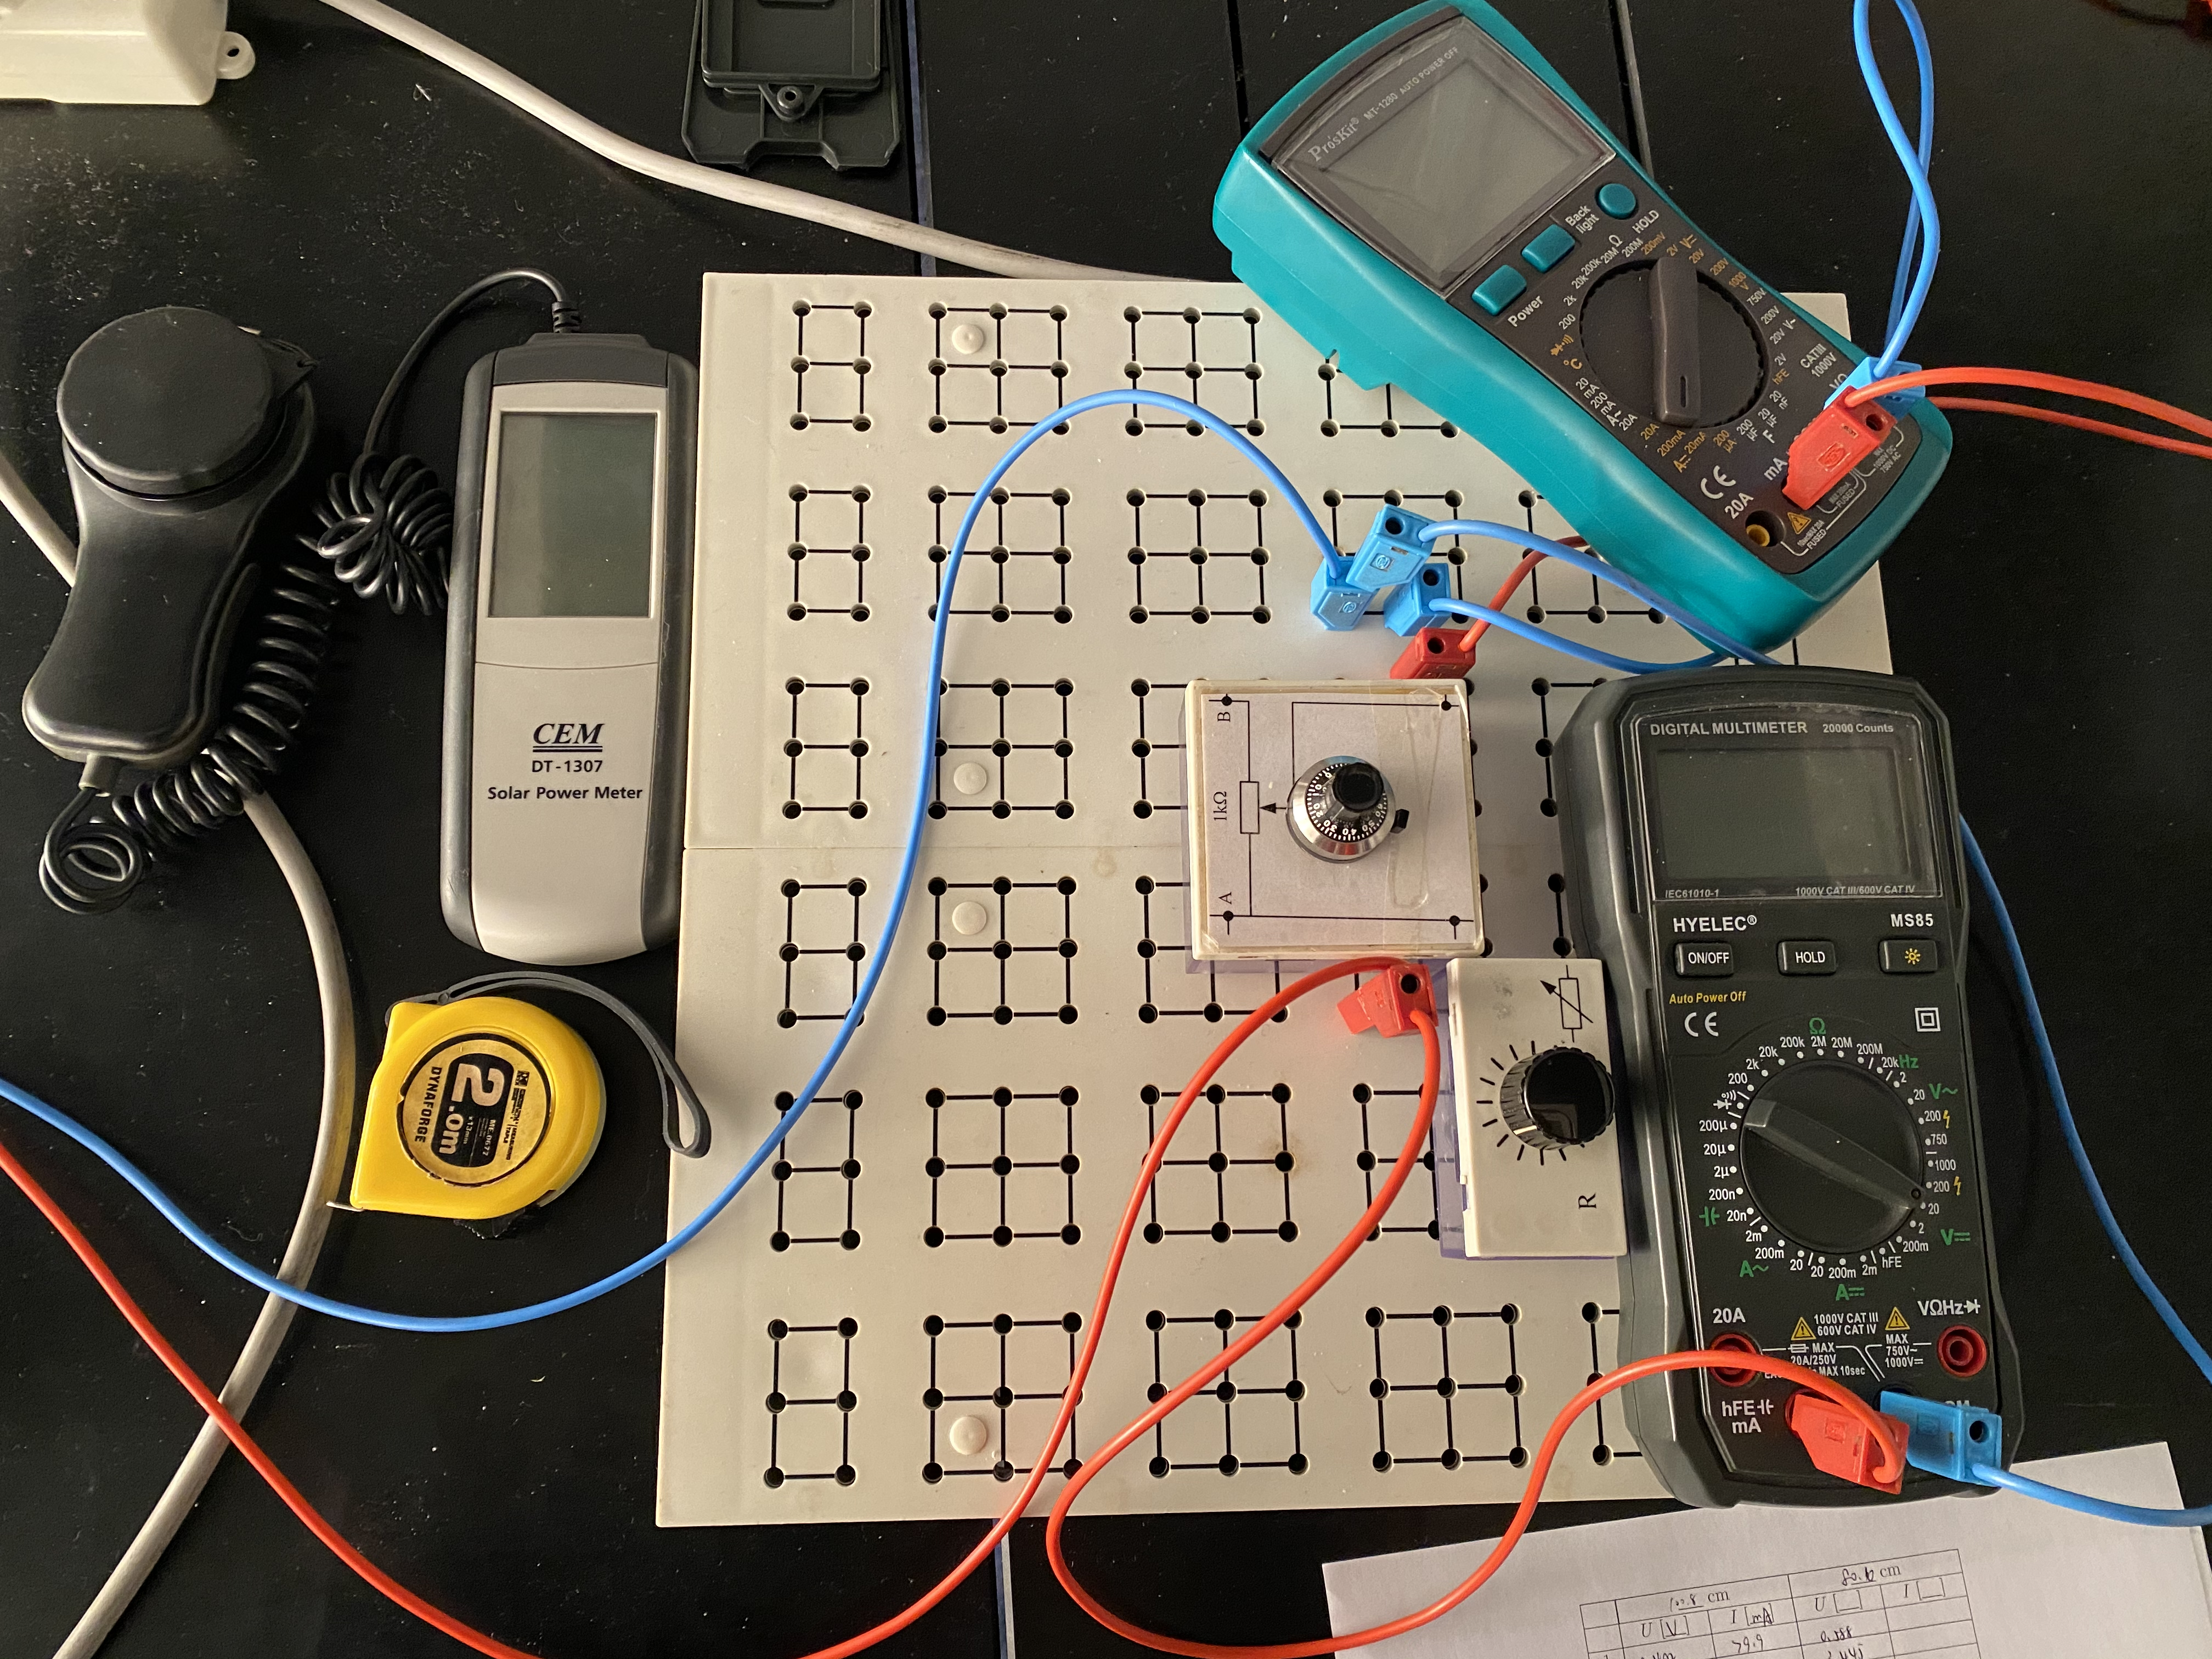
\includegraphics[width=6cm]{apparatus.jpg}
    }
    \caption{Apparatus}
\end{figure}
\begin{table}[H]
    \centering
    \begin{tabular}{|c|c|c|}
    \hline
    \textbf{Apparatus} & \textbf{Minimum Scale} &\textbf{Uncertainty} \\ \hline
    DC Voltage multimeter & 0.01V & $\pm$0.5\%+0.01V \\ \hline
    DC Current multimeter & 0.1mA & $\pm$0.5\%+0.1mA \\ \hline
    Measuring tape & 0.1cm & $\pm$0.1cm \\ \hline
    Solar power meter & 0.1$W/m^2$ & $\pm$10$W/m^2$ \\ \hline
    \end{tabular}
    \caption{Apparatus Information}
    \label{apparatus}
\end{table} 

\subsection{Measurement Procedure}
First, open light and fan. Measure the surface area of solar cell and the distance between light and the cell. Cooperate with other groups. Make two device of similar $I_{sc}$ and $V_{oc}$. Directly, put the multimeters on the solar cell to test $I_{sc}$ and $V_{oc}$ for series, parallel and different distances for single apparatus. And meadure $P_{in}$ at several places to get average value. Change the load resistance and get respectively current and voltage. Calculate P and R. Draw corresponding I-V and P-V and P-R plot of series, parallel, and single device of different distances. Finally, get "Isc; Voc; Pm; Im; Vm;Rm, FF, and $\eta$"[1]. 

\subsubsection{Caution}
While making the experiment, we should not touch the light in the same series of experiment to get constant light intensity.


\section{Result}
\subsection{Multimeter precision}
\begin{table}[H]
    \centering
    \begin{tabular}{|c|c|}
    \hline
    QUANTITY    & PRECISION \\ \hline
    DC voltage  & $\pm(0.5\%+0.01)V$ \\ \hline
    DC current  & $\pm(0.5\%+0.1)mA$ \\ \hline
    Distance    & $\pm 0.1cm$ \\ \hline
    Solar power & $\pm 10W/m^2$ \\ \hline
    \end{tabular}
    \caption{Multimeter precision}
\end{table}

\subsection{Measurement of $P_{in}$}
\subsubsection{Measurement of area}
We have measured the length and width of the cell (black area):
\begin{table}[H]
    \centering
    \begin{tabular}{|c|c|}
    \hline
    Length{[}cm{]} & Width{[}cm{]} \\ \hline
    25.9$\pm$0.1  & 21.2$\pm$0.1  \\ \hline
    \end{tabular}
    \caption{Measurement data for area}
\end{table}
Then we calculate the surface area of the solar cell:
$$A=ab=0.259\times 0.212=0.05491\pm 0.0003m^2$$

\subsubsection{Measurement of solar power}
We have measure six different place on the solar cell, 100.8cm and 80.6cm respectively from the solar cell:
\begin{table}[H]
    \centering
    \begin{tabular}{|c|c|c|c|c|c|c|}
    \hline
      & 1   & 2   & 3   & 4   & 5   & 6   \\ \hline
    $P_{100.8}[W/m^2]$ & 235 & 240 & 232 & 225 & 250 & 263 \\ \hline
    $P_{80.6}[W/m^2]$ & 345 & 358 & 346 & 374 & 712 & 648 \\ \hline
    \end{tabular}
    \caption{Measurement data for solar power}
\end{table}

Then we can calculate the average solar power at respectively 100.8cm and 80.6cm:
\begin{equation*}
    \overline{P_{100.8}}=\frac{235+240+232+225+250+263}{6}=241\pm14W/m^2
\end{equation*}

\begin{equation*}
    \overline{P_{80.6}}=\frac{345+358+346+374+712+648}{6}=4.60\pm1.7\times 10^2 W/m^2
\end{equation*}

\subsubsection{Caculation of Input Power $P_{in}$}
\begin{equation*}
    P_{in,100.8}=\overline{P_{100.8}}\times A241\times0.05491=13\pm1W
\end{equation*}

\begin{equation*}
    P_{in,80.6}=\overline{P_{80.6}}\times A=25\pm 5 W
\end{equation*}

\subsection{Measurement of $U_{oc}$ and $I_{sc}$}
\begin{table}[H]
    \centering
    \begin{tabular}{|c|c|c|c|c|}
    \hline
       & Single device at 100.8cm & Single device at 80.6cm & series & parallel \\ \hline
    $U_{oc}$[V]  & 10.01  & 10.43 & 19.84  & 9.89  \\ \hline
    $u_{U_{oc}}$[V] & 0.06 & 0.06  & 0.11  & 0.06 \\ \hline
    $I_{sc}$[mA]  & 80.4 & 118.2 & 82.6 & 166.2  \\ \hline
    $u_{I_{sc}}$[mA] & 0.5 & 0.7 & 0.5  & 0.9 \\ \hline
    \end{tabular}
    \caption{Measurement data for $u_{oc}$ and $I_{sc}$}
\end{table}

\subsection{ Measurement of U and I relations of 4 types and their corresponding P and R}
By using $P=UI$ and $R=\frac{U}{I}$, we can get the data of following four tables.

\begin{table}[H]
    \centering
    \begin{tabular}{|c|c|c|c|c|c|c|c|}
    \hline
    U{[}V{]} & $u_U$[V] & I{[}mA{]} & $u_I$[mA] & P[mW] & $u_P$[mW] & R[k$\Omega$] & $u_R$[k$\Omega$] \\ \hline
    0.660    & 0.013 & 82.3      & 1.3 & 54.3 & 1.4 & 0.0080 & 0.0002 \\ \hline
    3.01     & 0.03  & 81.0      & 1.3 & 244  & 4   & 0.0372 & 0.0007 \\ \hline
    5.49     & 0.04  & 79.3      & 1.3 & 435  & 8   & 0.0692 & 0.0012 \\ \hline
    7.28     & 0.05  & 78.2      & 1.3 & 569  & 10  & 0.0931 & 0.0016 \\ \hline
    9.70     & 0.06  & 75.0      & 1.2 & 728  & 13  & 0.129  & 0.002  \\ \hline
    9.97     & 0.06  & 74.7      & 1.2 & 744  & 13  & 0.133  & 0.002  \\ \hline
    10.93    & 0.06  & 73.1      & 1.2 & 799  & 14  & 0.149  & 0.003  \\ \hline
    11.95    & 0.07  & 71.4      & 1.2 & 853  & 15  & 0.167  & 0.003  \\ \hline
    12.75    & 0.07  & 70.2      & 1.2 & 895  & 16  & 0.182  & 0.003  \\ \hline
    13.66    & 0.08  & 67.4      & 1.1 & 920  & 16  & 0.203  & 0.004  \\ \hline
    14.51    & 0.08  & 64.4      & 1.1 & 934  & 16  & 0.225  & 0.004  \\ \hline
    15.01    & 0.09  & 62.3      & 1.0 & \textbf{935}  & 16  & 0.241  & 0.004  \\ \hline
    15.69    & 0.09  & 59.0      & 1.0 & 926  & 16  & 0.266  & 0.005  \\ \hline
    15.92    & 0.09  & 57.6      & 1.0 & 917  & 16  & 0.276  & 0.005  \\ \hline
    16.06    & 0.09  & 56.5      & 0.9 & 908  & 16  & 0.284  & 0.005  \\ \hline
    16.36    & 0.09  & 54.5      & 0.9 & 891  & 16  & 0.300  & 0.005  \\ \hline
    16.74    & 0.09  & 51.4      & 0.9 & 860  & 15  & 0.326  & 0.006  \\ \hline
    16.87    & 0.09  & 50.1      & 0.9 & 845  & 15  & 0.337  & 0.006  \\ \hline
    17.45    & 0.10  & 44.4      & 0.8 & 775  & 14  & 0.393  & 0.007  \\ \hline
    17.93    & 0.10  & 38.8      & 0.7 & 695  & 13  & 0.462  & 0.009  \\ \hline
    18.09    & 0.10  & 36.4      & 0.6 & 659  & 12  & 0.497  & 0.009  \\ \hline
    18.51    & 0.10  & 29.8      & 0.5 & 552  & 11  & 0.621  & 0.012  \\ \hline
    18.94    & 0.10  & 21.8      & 0.4 & 413  & 8   & 0.869  & 0.018  \\ \hline
    19.06    & 0.11  & 19.2      & 0.4 & 366  & 8   & 0.99   & 0.02   \\ \hline
    19.12    & 0.11  & 17.6      & 0.4 & 337  & 7   & 1.09   & 0.02   \\ \hline
    \end{tabular}
    \caption{Calculation of P and R of series connection}
\end{table}

\begin{table}[H]
    \centering
    \begin{tabular}{|c|c|c|c|c|c|c|c|}
    \hline
    U{[}V{]} & $u_U$[V] & I{[}mA{]} & $u_I$[mA] & P[mW] & $u_P$[mW] & R[k$\Omega$] & $u_R$[k$\Omega$]\\ \hline
    9.82    & 0.06 & 9.0       & 0.2 & 88  & 2  & 1.09    & 0.03    \\ \hline
    9.75    & 0.06 & 16.9      & 0.4 & 165 & 4  & 0.577   & 0.013   \\ \hline
    9.68    & 0.06  & 24.6      & 0.5 & 238 & 5  & 0.393   & 0.008   \\ \hline
    9.62    & 0.06  & 30.3      & 0.6 & 291 & 6  & 0.317   & 0.006   \\ \hline
    9.51    & 0.06  & 40.1      & 0.7 & 381 & 7  & 0.237   & 0.004   \\ \hline
    9.37    & 0.06  & 51.3      & 0.9 & 481 & 9  & 0.183   & 0.003   \\ \hline
    9.21    & 0.06  & 62.4      & 1.0 & 575 & 10 & 0.148   & 0.003   \\ \hline
    9.02    & 0.06  & 74.1      & 1.2 & 669 & 12 & 0.122   & 0.002   \\ \hline
    8.83    & 0.05  & 83.8      & 1.4 & 740 & 13 & 0.1054  & 0.0018  \\ \hline
    8.76    & 0.05  & 87.3      & 1.4 & 765 & 13 & 0.1003  & 0.0017  \\ \hline
    8.72    & 0.05  & 88.9      & 1.4 & 775 & 13 & 0.0981  & 0.0017  \\ \hline
    8.67    & 0.05  & 91.2      & 1.5 & 791 & 14 & 0.0951  & 0.0016  \\ \hline
    8.39    & 0.05  & 102.1     & 1.6 & 856 & 15 & 0.0821  & 0.0014  \\ \hline
    8.01    & 0.05  & 113.9     & 1.8 & 912 & 16 & 0.0703  & 0.0012  \\ \hline
    7.50    & 0.05  & 125       & 2   & \textbf{938} & 16 & 0.0600  & 0.0010  \\ \hline
    7.10    & 0.05  & 131       & 2   & 933 & 16 & 0.0541  & 0.0009  \\ \hline
    6.91    & 0.05 & 134       & 2   & 925 & 16 & 0.0517  & 0.0009  \\ \hline
    6.77    & 0.04 & 135       & 2   & 917 & 16 & 0.0500  & 0.0009  \\ \hline
    6.41    & 0.04 & 140       & 2   & 896 & 15 & 0.0459  & 0.0008  \\ \hline
    5.64    & 0.04 & 146       & 2   & 825 & 14 & 0.0386  & 0.0007  \\ \hline
    4.77    & 0.03 & 152       & 2   & 723 & 12 & 0.0315  & 0.0005  \\ \hline
    3.79    & 0.03 & 156       & 2   & 589 & 10 & 0.0244  & 0.0004  \\ \hline
    2.93    & 0.03 & 159       & 2   & 465 & 8  & 0.0185  & 0.0003  \\ \hline
    2.00    & 0.02 & 162       & 3   & 324 & 6  & 0.0124  & 0.0002  \\ \hline
    0.974    & 0.015 & 165       & 3   & 161 & 4  & 0.00589 & 0.00013 \\ \hline
    \end{tabular}
    \caption{ Calculation of P and R for parallel connection}
\end{table}

\begin{table}[H]
    \centering
    \begin{tabular}{|c|c|c|c|c|c|c|c|}
    \hline
    U{[}V{]} & $u_U$[V] & I{[}mA{]} & $u_I$[mA] & P[mW] & $u_P$[mW] & R[k$\Omega$] & $u_R$[k$\Omega$]\\ \hline
    0.402    & 0.012 & 79.9      & 1.3 & 32.1 & 1.1 & 0.00503 & 0.00017 \\ \hline
    2.00     & 0.02  & 79.1      & 1.3 & 159  & 3   & 0.0253 & 0.0005 \\ \hline
    4.54     & 0.03  & 75.2      & 1.2 & 342  & 6   & 0.0604 & 0.0011 \\ \hline
    6.68     & 0.04  & 70.5      & 1.2 & 471  & 8   & 0.0947 & 0.0017 \\ \hline
    7.18     & 0.05  & 69.3      & 1.1 & 498  & 9   & 0.1036 & 0.0018 \\ \hline
    7.21     & 0.05  & 69.1      & 1.1 & 498  & 9   & 0.1043 & 0.0018 \\ \hline
    7.36     & 0.05  & 68.2      & 1.1 & 502  & 9   & 0.1079 & 0.0019 \\ \hline
    7.53     & 0.05  & 67.3      & 1.1 & 507  & 9   & 0.112  & 0.002  \\ \hline
    7.79     & 0.05  & 65.8      & 1.1 & \textbf{513}  & 9   & 0.118  & 0.002  \\ \hline
    7.89     & 0.05  & 64.1      & 1.1 & 505  & 9   & 0.123  & 0.002  \\ \hline
    8.02     & 0.05  & 62.6      & 1.0 & 502  & 9   & 0.128  & 0.002  \\ \hline
    8.05     & 0.05  & 61.5      & 1.0 & 495  & 9   & 0.131  & 0.002  \\ \hline
    8.36     & 0.05  & 57.6      & 1.0 & 481  & 9   & 0.145  & 0.003  \\ \hline
    8.60     & 0.05  & 53.7      & 0.9 & 462  & 8   & 0.160  & 0.003  \\ \hline
    8.88     & 0.05  & 48.3      & 0.8 & 429  & 8   & 0.184  & 0.003  \\ \hline
    9.02     & 0.06  & 45.2      & 0.8 & 408  & 7   & 0.200  & 0.004  \\ \hline
    9.15     & 0.06  & 41.9      & 0.7 & 384  & 7   & 0.218  & 0.004  \\ \hline
    9.26     & 0.06  & 38.8      & 0.7 & 359  & 7   & 0.239  & 0.004  \\ \hline
    9.36     & 0.06  & 35.7      & 0.6 & 334  & 6   & 0.262  & 0.005  \\ \hline
    9.50     & 0.06  & 30.6      & 0.6 & 291  & 6   & 0.310  & 0.006  \\ \hline
    9.62     & 0.06  & 25.6      & 0.5 & 246  & 5   & 0.376  & 0.007  \\ \hline
    9.72     & 0.06  & 20.6      & 0.4 & 200  & 4   & 0.472  & 0.010  \\ \hline
    9.82     & 0.06  & 15.4      & 0.3 & 151  & 3   & 0.637  & 0.014  \\ \hline
    9.90     & 0.06  & 10.8      & 0.3 & 107  & 3   & 0.92   & 0.02   \\ \hline
    9.93     & 0.06  & 8.0       & 0.2 & 79   & 2   & 1.24   & 0.03   \\ \hline
    \end{tabular}
    \caption{Calculation of P and R for single device at 100.8cm}
\end{table}

\begin{table}[H]
    \centering
    \begin{tabular}{|c|c|c|c|c|c|c|c|}
    \hline
    U{[}V{]} & $u_U$[V] & I{[}mA{]} & $u_I$[mA] & P[mW] & $u_P$[mW] & R[k$\Omega$] & $u_R$[k$\Omega$] \\ \hline
    0.588    & 0.013 & 118.6     & 1.9 & 69.7 & 1.9 & 0.00496 & 0.00013 \\ \hline
    3.45     & 0.03  & 115.2     & 1.8 & 397  & 7   & 0.0299 & 0.0005 \\ \hline
    4.63     & 0.03  & 113.7     & 1.8 & 526  & 9   & 0.0407 & 0.0007 \\ \hline
    5.65     & 0.04  & 112.6     & 1.8 & 636  & 11  & 0.0502 & 0.0009 \\ \hline
    6.02     & 0.04  & 111.7     & 1.8 & 672  & 12  & 0.0538 & 0.0009 \\ \hline
    7.52     & 0.05  & 104.3     & 1.7 & 784  & 13  & 0.0721 & 0.0012 \\ \hline
    7.75     & 0.05  & 102.2     & 1.6 & 792  & 14  & 0.0758 & 0.0013 \\ \hline
    7.95     & 0.05  & 100.1     & 1.6 & 796  & 14  & 0.0794 & 0.0014 \\ \hline
    8.19     & 0.05  & 97.4      & 1.6 & \textbf{798}  & 14  & 0.0841 & 0.0014 \\ \hline
    8.37     & 0.05  & 94.6      & 1.5 & 792  & 14  & 0.0885 & 0.0015 \\ \hline
    8.53     & 0.05  & 92.4      & 1.5 & 788  & 14  & 0.0923 & 0.0016 \\ \hline
    8.72     & 0.05  & 88.4      & 1.4 & 771  & 13  & 0.0987 & 0.0017 \\ \hline
    8.93     & 0.05  & 83.9      & 1.4 & 749  & 13  & 0.1064 & 0.0018 \\ \hline
    9.12     & 0.06  & 79.3      & 1.3 & 724  & 13  & 0.115  & 0.002  \\ \hline
    9.20     & 0.06  & 76.1      & 1.2 & 700  & 12  & 0.121  & 0.002  \\ \hline
    9.36     & 0.06  & 70.3      & 1.2 & 658  & 12  & 0.133  & 0.002  \\ \hline
    9.45     & 0.06  & 66.6      & 1.1 & 629  & 11  & 0.142  & 0.002  \\ \hline
    9.54     & 0.06  & 62.8      & 1.0 & 599  & 11  & 0.152  & 0.003  \\ \hline
    9.63     & 0.06  & 58.1      & 1.0 & 560  & 10  & 0.166  & 0.003  \\ \hline
    9.75     & 0.06  & 51.7      & 0.9 & 504  & 9   & 0.189  & 0.003  \\ \hline
    9.85     & 0.06  & 45.4      & 0.8 & 447  & 8   & 0.217  & 0.004  \\ \hline
    10.01    & 0.06  & 33.8      & 0.6 & 338  & 6   & 0.296  & 0.006  \\ \hline
    10.15    & 0.06  & 22.0      & 0.4 & 223  & 5   & 0.461  & 0.009  \\ \hline
    10.22    & 0.06  & 16.2      & 0.3 & 166  & 4   & 0.631  & 0.014  \\ \hline
    10.28    & 0.06  & 9.9       & 0.2 & 102  & 3   & 1.04   & 0.03   \\ \hline
    \end{tabular}
    \caption{Calculation of P and R for single device at 80.6cm}
\end{table}

Then we can plot I-U, P-U, and P-R as follow.
\begin{figure}[H]
    \centering
    \includegraphics[width=9cm]{ui.png}
    \caption{I-V characteristic}
\end{figure}

\begin{figure}[H]
    \centering
    \includegraphics[width=10cm]{up.png}
    \caption{P-U relation}
\end{figure}

\begin{figure}[H]
    \centering
    \includegraphics[width=10cm]{rp.png}
    \caption{P-R relation}
\end{figure}

\section{Calculation of FF and $\eta$}
\begin{equation*}
    FF=\frac{P_m}{V_{oc}I_{sc}}
\end{equation*}
\begin{equation*}
    \eta=\frac{P_m}{P_{in}}\times100\%
\end{equation*}
For a single device at 100.8cm, $P_m=513\pm9mW=0.513\pm0.009W$, $V_{oc}=10.01\pm0.06V$, $I_{sc}=80.4\pm0.5mA=0.0804\pm0.0005A$
\begin{equation*}
    FF_{100.8cm}=\frac{P_m}{V_{oc}I_{sc}}=\frac{0.513}{10.01\times0.0804}=0.637\pm0.012
\end{equation*}
\begin{equation*}
    \eta_{100.8cm}=\frac{P_m}{P_{in}}\times100\%=\frac{0.513}{13}\times100\%=4.0\%\pm0.3\%
\end{equation*}

For a single device at 80.6cm, $P_m=798\pm14mW=0.798\pm0.014W$, $V_{oc}=10.43\pm0.06V$, $I_{sc}=118.2\pm0.7mA=0.1182\pm0.0007A$
\begin{equation*}
    FF_{80.6cm}=\frac{P_m}{V_{oc}I_{sc}}=\frac{0.798}{10.43\times0.1182}=0.65\pm0.04
\end{equation*}
\begin{equation*}
    \eta_{80.6cm}=\frac{P_m}{P_{in}}\times100\%=\frac{0.798}{25}\times100\%=3.2\%\pm0.6\%
\end{equation*}

And we can get following table:
\begin{table}[H]
    \centering
    \begin{tabular}{|c|c|c|c|c|}
    \hline
    & Series& Parallel & 100.8cm  & 80.6cm\\ \hline
    Voc[V] & 19.84$\pm$0.11 & 9.89$\pm$0.06 & 10.01$\pm$0.06  & 10.43$\pm$0.06  \\ \hline
    Isc[mA] & 82.6$\pm$0.5   & 166.2$\pm$0.9 & 80.4$\pm$0.5    & 118.2$\pm$0.7   \\ \hline
    Pm[mW]  & 935$\pm$16     & 938$\pm$16    & 513$\pm$9       & 798$\pm$14      \\ \hline
    Vm[V]  & 19.12$\pm$0.11 & 9.82$\pm$0.06 & 9.93$\pm$0.06   & 10.28$\pm$0.06 \\ \hline
    Im[mA]  & 82.3$\pm$1.3   & 165$\pm$3     & 79.9$\pm$1.3    & \textbf{118.6$\pm$1.9}   \\ \hline
    Rm[k$\omega$]  & 0.241$\pm$0.004  & 0.0600$\pm$0.0010 & 0.118$\pm$0.002   & 0.0841$\pm$0.0014   \\ \hline
    FF  & -  & - & 0.637$\pm$0.012 & 0.65$\pm$0.04   \\ \hline
    eta & -  & - & 4.0\%$\pm$0.3\% & 3.2\%$\pm$0.6\% \\ \hline
    \end{tabular}
    \caption{Experiment Result}
    \label{final}
\end{table}

\section{Conclusions}
We have learnt the principle of solar cell and its I-U characteristics. We have did following four series of experiment:
\begin{itemize}
    \item Two solar cells in series
    \item Two solar cells in parallel
    \item One solar cell at the distance 100.8cm from light source
    \item One solar cell at the distance 80.6cm from light source
\end{itemize}
Based on the calculated data and figures we plot, we can do some analysis, thus finding the most efficient usage. So, we can better use the solar energy and protect our environment. This is the significance of this experiment.\par
The solar cells in series and parallel have the same distance as single device at 100.8cm.
Through I-U plots and Table.\ref{final}, we can get the effect of different connections.
\begin{itemize}
    \item 	When sharing same voltage, the current through parallel cells doubled then one single cell.
    \item   When sharing same current, the voltage over parallel series doubled than one single cell.
    \item Parallel cells have similar $V_{oc}$ as one single device.
    \item Series cells have similar $I_{sc}$ as one single device.
    \item The $P_m$ of two different connections are almost the same, and they are doubled than single device.
    \item When we gwt $P_m$, series cell have doubled voltage while parallel cells have doubled current. $R_m$ of series cells doubles of single cell and is four times of parallel cells.
\end{itemize}
Also, there exists certain effect of distance.
\begin{itemize}
    \item 	When sharing same voltage, the current is connected to distance negatively.
    \item When sharing same current, the voltage is connected to distance positively.
	\item When distance increase, both $V_{oc}$ and $I_{sc}$ decrease.
	\item When distance increase, $P_m$ decreases and $R_m$ increases.
    \item With distance increase, FF decrease. This is because of smaller incident light.
\end{itemize}
The error may cause by following reasons.
\begin{itemize}
    \item In Table.\ref{final}, we see fourth line have larger currents than the $I_{sc}$ measured previously. This might because of neighboring groups moved their light source, thus changing the light intensity.
    \item In Table.\ref{final}, we can find one value of resistor is bigger than 1.1$k\Omega$, this may because of the wrongly measured current. Since current then is so small that it will be effected at a large range.
    \item Sheltering the light source accidentally may also cause errors.
    \item Light non-uniformly incident on the solar cell, which causes inaccuracy of calculation of $P_{in}$.
    \item The inner resistance of multimeters, which causes error in current and voltage.
\end{itemize}
We can do following to help improve the accuracy
\begin{itemize}
    \item Find an environment with stable light source.
	\item Do more set of experiments to make contrasts.
\end{itemize}


\section{Reference}
[1] Qin Tian, Feng Yaming, Gu Yichen, Mateusz Krzyzosiak. Physics Laboratory VP241 Ex-
ercise 5: RC, RL, and RLC Circuits.


\newpage
{\LARGE\textbf{APPENDIX}}
\setcounter{section}{0}
\renewcommand\thesection{\Alph{section}}
\section{Data Sheet}

\end{document}